\documentclass[english]{article}

\usepackage{graphicx}
\usepackage{alltt}
\usepackage{url}
\usepackage{tabularx}
%\usepackage{ngerman}
\usepackage{longtable}
\usepackage{color}

\usepackage{xifthen}
\newboolean{showbackdoors}
\setboolean{showbackdoors}{true}  % set to false to hide subsection on backdoors for reviewing group


\newenvironment{prettytablex}[1]{\vspace{0.3cm}\noindent\tabularx{\linewidth}{@{\hspace{\parindent}}#1@{}}}{\endtabularx\vspace{0.3cm}}
%\newenvironment{prettytable}{\prettytablex{l X}}{\endprettytablex}



\title{\huge\sffamily\bfseries System Description and Risk Analysis}
\author{Cyrill Krähenbühl \and Silvan Egli \and Lukas Bischofberger}
\date{\dots}


\begin{document}
\maketitle

%% **** please observe the page limit **** 
%% (it is not allowed to change the font size or page geometry to gain more space)
%% comment or remove lines below before hand-in
\begin{center}
{\large\textcolor{red}{Page limit: 30 pages.}}
\end{center}
%%%%%%%%%%%%%%%%%%%%%%%%%%%%%%%%%%%%%%%%%%%%%%

\tableofcontents
\pagebreak


\section{System Characterization}

\subsection{System Overview}

20 points

\begin{figure}[ht]
	\centering
	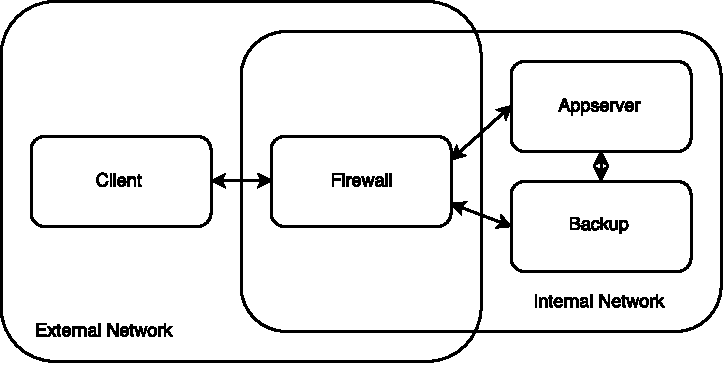
\includegraphics[scale=0.7]{systemoverview.pdf}
	\caption{System overview}
	\label{figure:systemoverview}
\end{figure}

Describe the system's mission,  the system boundaries,
and the overall system architecture, including the main subsystems and
their relationships.   This description should provide a high-level
overview of the system, e.g., suitable for managers, that complements
the more technical description that follows.


\subsection{System Functionality}

Describe the system's functions.


\subsection{Security Design}

Describe the system's security design, including key and session management and 
security of data at rest and in transit.


\subsection{Components}

List all system components and their interfaces, subdivided, for example, into
  categories such as platforms, applications, data records, etc. For
  each component, state its relevant properties.


\ifthenelse{\boolean{showbackdoors}}{
% show for handed-in version

\subsection{Backdoors}

Describe the implemented backdoors. 

\bigskip\noindent
\textbf{Hide this subsection in the version handed over to the reviewing team by setting the flag \texttt{showbackdoors} at the top of this document to \texttt{false}.}


%% do not delete the three lines below
}{ 
% empty for reviewing group's version
} 

\subsection{Additional Material}

You may have additional sections according to your needs.


\section{Risk Analysis and Security Measures}

\subsection{Assets}

3 points

physical:

- firewall
- appserver
- backupserver
- internal network
- external network


logical:
- connectivity

software:
- firewall os
- firewall service
- appserver os
- appserver webserver
- appserver application
- appserver ca scripts
- backupserver os
- backupserver duplicity

information:
database
- certificates
- appserver application configuration (webserver, database, django, ca, ssh)
- private keys
- crl
- backupserver application config
- Logs
- Login credentials
- jwt
- archive key
- ca key (intermediate \& root key)


persons:
- user/employee
- ca administrator
- system administrator
- private key holder

intangible:
- user confidence

Describe the relevant assets and their required security
  properties. For example, data objects, access restrictions,
  configurations, etc.

\subsection{Threat Sources}

3 points

- Nature
- user
- system administrator
- script kiddies
- skilled hacker
- malware
- organized crime
- competitors (e.g. JMovie)

Name and describe potential threat sources including their motivation.

\subsection{Risks Definitions}

2 points

Define likelihood, impact and risk level using the following three
  tables.

%\subsubsection{Tools}

\begin{center}
\begin{table}[h]
\begin{tabularx}{\textwidth}{|l|X|}
\hline
\multicolumn{2}{|c|}{\bf Likelihood} \\
\hline
Likelihood & Description \\
\hline
\hline
High & The threat source is highly motivated and sufficiently capable of exploiting a given vulnerability in order to change the asset’s state. The controls to prevent the vulnerability from being exploited are ineffective.\\
\hline
Medium & The threat source is motivated and capable of exploiting a given vulnerability in order to change the asset’s state, but controls are in place that may impede a successful exploit of the vulnerability. \\
\hline
Low   & The threat source lacks motivation or capabilities to exploit a given vulnerability in order to change the asset’s state. Another possibility that results in a low likelihood is the case where controls are in place that prevent (or at least significantly impede) the vulnerability from being exercised. \\
\hline
\end{tabularx}
\end{table}
\hspace{3em}
\begin{table}[h]
\begin{tabularx}{\textwidth}{|l|X|}
\hline
\multicolumn{2}{|c|}{\bf Impact} \\
\hline
Impact & Description \\
\hline
\hline
High   & The event (1) may result in a highly costly loss of major tangible assets or resources; (2) may significantly violate, harm, or impede an organization’s mission, reputation, or interest; or (3) may result in human death or serious injury. \\
\hline
Medium & The event (1) may result in a costly loss of tangible assets or resources; (2) may violate, harm, or impede an organization’s mission, reputation, or interest, or (3) may result in human injury.\\
\hline
Low & The event (1) may result in a loss of some tangible assets or resources or (2) may noticeably affect an organization’s mission, reputation, or interest.\\
\hline
\end{tabularx}
\end{table}
\end{center}

\vspace{5mm}

\begin{center}
\begin{tabular}{|l|c|c|c|}
\hline
\multicolumn{4}{|c|}{{\bf Risk Level}} \\
\hline
{{\bf Likelihood}} & \multicolumn{3}{c|}{{\bf Impact}} \\ \cline{2-4}
     & Low & Medium & High \\  \hline
 High & Low & Medium & High  \\
\hline
 Medium & Low & Medium & Medium \\
\hline
 Low & Low & Low & Low \\
\hline
\end{tabular}
\end{center}


\subsection{Risk Evaluation}

7 points

List all potential threats and the corresponding countermeasures. Estimate the risk based on the information about the threat, the threat sources and the corresponding countermeasure. Adhere to the risk definitions you have given above.


\subsubsection{{\it Evaluation Asset X}}

Evaluate the likelihood, impact and the resulting risk,  \emph{after implementation of the corresponding countermeasures}. For each threat, clearly name the threat source and the the threat action.

\begin{footnotesize}
\begin{prettytablex}{llp{5.5cm}lll}
No. & Threat &  Countermeasure(s) & L & I & Risk \\
\hline
1 & ... & ... & {\it Low} & {\it Low} & {\it Low} \\
\hline
2 & ... & ...& {\it Medium} & {\it High} & {\it Medium} \\
\hline
\end{prettytablex}
\end{footnotesize}



\subsubsection{{\it Evaluation Asset y}}

\begin{footnotesize}
\begin{prettytablex}{llp{5.5cm}lll}
No. & Threat & Countermeasure(s) & L & I & Risk \\
\hline
1 & ... & ... & {\it Low} & {\it Low} & {\it Low} \\
\hline
2 & ... & ...& {\it Medium} & {\it High} & {\it Medium} \\
\hline
\end{prettytablex}
\end{footnotesize}

\subsubsection{Detailed Description of Selected Countermeasures}

Optionally explain the details of the countermeasures mentioned above.



\subsubsection{Risk Acceptance}

List all medium and high risks, according to the evaluation above. For each risk, propose additional countermeasures that could be implemented to further reduce the risks.

\begin{footnotesize}
\begin{prettytablex}{p{2cm}X}
No. of threat & Proposed additional countermeasure including expected impact  \\
\hline
... & ... \\
\hline
... & ... \\
\hline
\end{prettytablex}
\end{footnotesize}

\end{document}

%%% Local Variables: 
%%% mode: latex
%%% TeX-master: "../../book"
%%% End: 
